%
% system_overview.tex
%
% Copyright (C) 2021 by SpaceLab.
%
% Flatsat Platform Documentation
%
% This work is licensed under the Creative Commons Attribution-ShareAlike 4.0
% International License. To view a copy of this license,
% visit http://creativecommons.org/licenses/by-sa/4.0/.
%

%
% \brief System Overview chapter.
%
% \author Gabriel Mariano Marcelino <gabriel.marcelino@spacelab.ufsc.br>
% \author Yan Castro de Azeredo <yan.azeredo@spacelab.ufsc.br>
%
% \institution Universidade Federal de Santa Catarina (UFSC)
%
% \version 0.1.0
%
% \date 2020/12/17
%

\chapter{System Overview} \label{ch:system-overview}

The FlatSat form factor choosen for this project is a retangular one piece design. On its current version v0.1 the platform can be purelly used hardware wise. The hardware block diagram can be seen on \autoref{fig:block-diagram}. The PC-104 slot N$^{\circ}$7 is supossed to be used for a extra interface, shield or another FlatSat platform.

\section{Block Diagram}

\begin{figure}[!ht]
    \begin{center}
        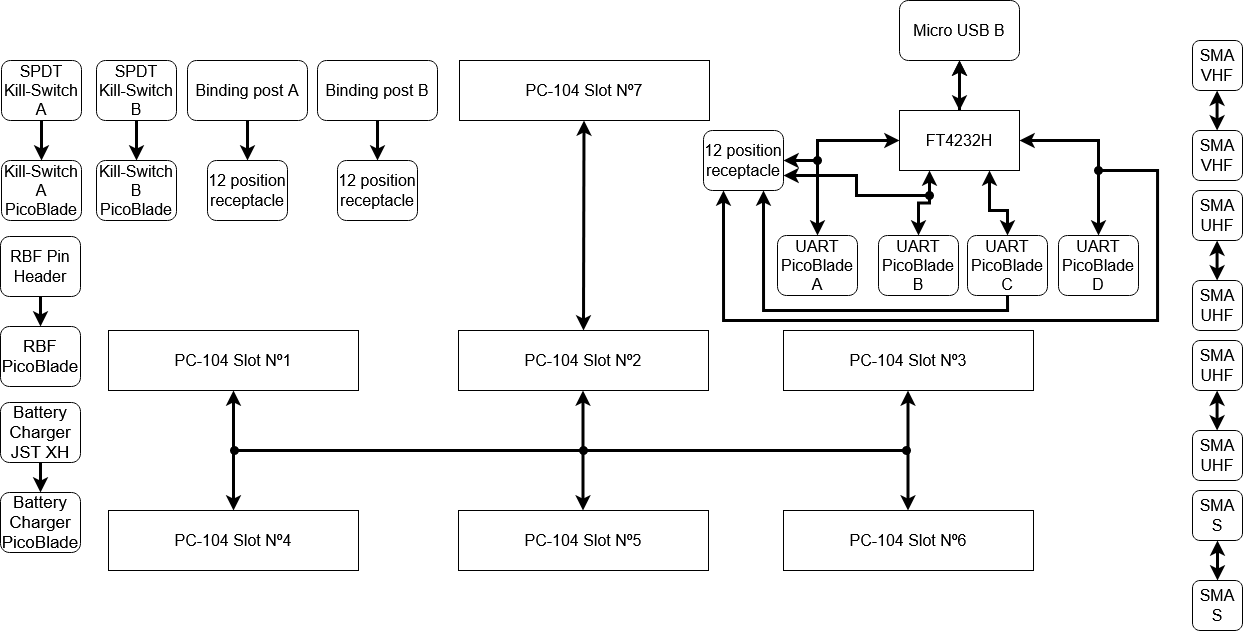
\includegraphics[width=\textwidth]{figures/flatsat_block_diagram.png}
        \caption{FlatSat hardware block diagram.}
        \label{fig:block-diagram}
    \end{center}
\end{figure}

\section{Board Dimensions}

The board is a retangular PCB with linear dimensions of 300$\times$220 mm. The full mechanical specs of the platform can be seen on its draftsman document available at it's GitHub repository \cite{flatsat-draftsman}.
